\documentclass[11pt]{article}
\usepackage[scaled=0.92]{helvet}
\usepackage{geometry}
\geometry{letterpaper,tmargin=1in,bmargin=1in,lmargin=1in,rmargin=1in}
\usepackage[parfill]{parskip} % Activate to begin paragraphs with an empty line rather than an indent %\usepackage{graphicx}
\usepackage{amsmath,amssymb, mathrsfs,  mathtools, dsfont}
\usepackage{tabularx}
\usepackage{tikz-cd}
\usepackage[font=footnotesize,labelfont=bf]{caption}
\usepackage{graphicx}
\usepackage{xcolor}
%\usepackage[linkbordercolor ={1 1 1} ]{hyperref}
%\usepackage[sf]{titlesec}
\usepackage{natbib}
\usepackage{../../Tianpei_Report}

%\usepackage{appendix}
%\usepackage{algorithm}
%\usepackage{algorithmic}

%\renewcommand{\algorithmicrequire}{\textbf{Input:}}
%\renewcommand{\algorithmicensure}{\textbf{Output:}}



\begin{document}
\title{Lecture 3: Countability and Separation Axioms}
\author{ Tianpei Xie}
\date{Nov. 7th., 2022}
\maketitle
\tableofcontents
\newpage
\section{The Countability and Separation Axioms}
\subsection{The Countability Axioms}
\begin{itemize}
\item \begin{definition} (\emph{\textbf{First-Countable}})\\
A space $X$ is said to have a \underline{\emph{\textbf{countable basis at $x$}}} if there is a \emph{\textbf{countable} collection} $\srB$ of \emph{\textbf{neighborhoods}} of $x$ such that \emph{each neighborhood} of $x$ \emph{\textbf{contains at least one}} of the elements of $\srB$. 

A space that has \emph{a \textbf{countable basis} at each of its points} is said to satisfy \underline{\emph{\textbf{the first countability}}} \underline{\emph{\textbf{axiom}}}, or to be \underline{\emph{\textbf{first-countable}}}.
\end{definition}

\item \begin{remark}
\emph{Every metric space is first-countable.}
\end{remark}

\item \begin{proposition} (\textbf{Limit Point Detected by Convergent Sequence}) \citep{munkres2000topology}\\
Let $X$ be a topological space.
\begin{enumerate}
\item Let $A$ be a subset of $X$. If there is a sequence of points of $A$ converging to $x$, then $x \in \bar{A}$; the \textbf{converse} holds if $X$ is \textbf{first-countable}.
\item Let $f : X \rightarrow Y$. If $f$ is continuous, then for every convergent sequence $x_n \rightarrow x$ in $X$, the sequence $f(x_n)$ converges to $f(x)$. The \textbf{converse} holds if X is \textbf{first-countable}.
\end{enumerate}
\end{proposition}

\item \begin{definition} (\emph{\textbf{Second-Countable}})\\
If a space $X$ has \emph{\textbf{a countable basis} for its topology}, then $X$ is said to satisfy \underline{\emph{\textbf{the second}}} \underline{\emph{\textbf{countability axiom}}}, or to be \underline{\emph{\textbf{second-countable}}}.
\end{definition}

\item \begin{example} ($\bR$)\\
The real line $\bR$ has a \emph{\textbf{countable basis}}, which is the collection of all \emph{open intervals} $(a, b)$ with \emph{\textbf{rational end points}}.
\end{example}

\item \begin{example} ($\bR^n$ and $\bR^{\omega}$ under \emph{product topology})
\begin{enumerate}
\item \emph{The finite dimensional space} $\bR^n$ has a \emph{\textbf{countable basis}}, which is the collection of all \emph{product of intervals}  with \emph{\textbf{rational end points}}.
\item \emph{The countable infinite dimensional space} $\bR^\omega$ has a \emph{\textbf{countable basis}}, which is the
collection of all products $\prod_{n\in \bZ_{+}} U_n$, where $U_n$ is an \emph{open interval with \textbf{rational end points}} \emph{for \textbf{finitely many} values} of $n$, and $U_n = \bR$ for \emph{all other values} of $n$.
\end{enumerate}
\end{example}

\item \begin{example}  (\emph{$\bR^{\omega}$ under \textbf{Uniform Topology} \textbf{Not Second-Countable}})\\
In the \emph{\textbf{uniform topology}}, $\bR^{\omega}$ satisfies \emph{the first countability axiom (being metrizable)}. However, it \emph{does \textbf{not satisfy the second}}. 

To verify this fact, we first show that if $X$ is a space having a countable basis $\srB$, then \emph{\textbf{any discrete subspace}} $A$ of $X$ must be \emph{\textbf{countable}}. Choose, for each $a \in A$, a basis element $B_a$ that \emph{intersects} $A$ in the point $a$ \emph{\textbf{alone}}. If $a$ and $b$ are distinct points of $A$, the sets $B_a$ and $B_b$ are \emph{different}, since the first \emph{contains} $a$ and the second does not. It follows that the map $a \mapsto
 B_a$ is an \emph{\textbf{injection}} of $A$ into $\srB$, so \emph{$A$ must be countable} (as $\srB$ being countable).
 
Now we note that the subspace $A$ of $\bR^{\omega}$ consisting of \emph{all sequences of $0$'s and $1$'s is \textbf{uncountable}}; and it has the \emph{\textbf{discrete topology}} because $\bar{\rho}(a, b) = 1$ for any two distinct points $a$ and $b$ of $A$. Therefore, in the uniform topology $\bR^{\omega}$ \emph{does not have a countable basis}. \qed
\end{example}

\item \begin{example} (\emph{\textbf{Topological Manifolds}})
 \begin{definition}
Suppose $M$ is a \emph{\textbf{topological space}}. We say that $M$ is a \underline{\emph{\textbf{topological manifold}}} of \emph{dimension $n$} or a \emph{\textbf{topological $n$-manifold}} if it has the following properties:
\begin{enumerate}
\item $M$ is a \emph{\textbf{Hausdorff space}}: for every pair of distinct points $p, q \in M$, there are disjoint open subsets $U, V \subseteq M$ such that $p \in U$ and $q \in V$.
\item $M$ is \emph{\textbf{second-countable}}: there exists a \emph{\textbf{countable basis}} for the topology of $M$.
\item $M$ is \emph{\textbf{locally Euclidean of dimension}} $n$: each point of $M$ has a neighborhood that is \emph{\textbf{homeomorphic}} to an open subset of $\bR^n$. 
\end{enumerate}
\end{definition}
\end{example}

\item Both countability axioms are well behaved with respect to the operations of taking subspaces or countable products:
\begin{proposition}(\textbf{Subspaces and Countable Product}) \citep{munkres2000topology}\\
A \textbf{subspace} of \rule{1cm}{0.0001mm}
\begin{enumerate}
\item a first-countable space is first-countable;
\item a second-countable space is second-countable.
\end{enumerate}
And a \textbf{countable product} of \rule{1cm}{0.0001mm}
\begin{enumerate}
\item first-countable spaces is first-countable;
\item second-countable spaces is second-countable.
\end{enumerate}
\end{proposition}

\item \begin{definition} (\emph{\textbf{Dense Subset}})\\
A subset $A$ of a space $X$ is said to be \underline{\emph{\textbf{dense}}} in $X$ if $\bar{A}=X$. (That is, \emph{every point in $X$ is a limit point of $A$.})
\end{definition}

\item \begin{definition} (\emph{\textbf{Separability}})\\
A topological space $X$ is called \underline{\emph{\textbf{separable}}} if and only if it has a \emph{\textbf{countable dense set}}.
\end{definition}

\item \begin{definition} (\emph{\textbf{Lindel{\"o}f Space}})\\
A space for which \emph{every open covering} contains \emph{a \textbf{countable} subcovering} is called a \underline{\emph{\textbf{Lindel{\"o}f space}}}. 
\end{definition}

\item \begin{proposition} (\textbf{Properties of Second-Countability}) \citep{munkres2000topology}\\
Suppose that $X$ has a \textbf{countable basis}. Then:
\begin{enumerate}
\item Every \textbf{open covering} of $X$ contains a \textbf{countable} subcollection covering $X$. ($X$ is \textbf{Lindel{\"o}f space})
\item There exists a \textbf{countable} subset of $X$ that is \textbf{dense} in $X$. ($X$ is \textbf{separable})
\end{enumerate}
\end{proposition}

\item \begin{proposition}  (\textbf{Metric Space Equivalence}) \citep{munkres2000topology}\\
Suppose that $X$ is a \textbf{metrizable spcae}. The following statements are equivalent: 
\begin{enumerate}
\item $X$ has a \textbf{countable basis} (\textbf{second-countable}).
\item $X$ has a \textbf{countable dense subset} (\textbf{separable}).
\item Every \textbf{open covering} of $X$ contains a \textbf{countable} subcollection covering $X$. (\textbf{Lindel{\"o}f space}).
\end{enumerate}
\end{proposition}

\item \begin{proposition}  (\textbf{Compact Metrizable Space}) \citep{munkres2000topology}\\
Every \textbf{compact metrizable} space $X$ has a countable basis (i.e. \textbf{second-countable}). 
\end{proposition} [Hint: Let $\srA_n$ be a finite covering of $X$ by $1/n$-balls.]

\item \begin{proposition} (\textbf{Preservation by Continuity}) \citep{munkres2000topology}\\
Let $f : X \rightarrow Y$ be continuous. 
\begin{enumerate}
\item If $X$ is \textbf{Lindel{\"o}f }, then $f(X)$ is \textbf{Lindel{\"o}f };
\item if $X$ has a \textbf{countable dense subset}, then $f(X)$ satisfies the same condition.
\end{enumerate}
\end{proposition}

\item \begin{proposition}(\textbf{Preservation by Product}) \citep{munkres2000topology}\\
If $X$ is a \textbf{countable product} of spaces having countable dense subsets (\textbf{separable}), then $X$ has a countable dense subset (\textbf{separable}). 
\end{proposition}

\item \begin{example} (\emph{\textbf{The Product of two Lindel{\"o}f Spaces Need Not be Lindel{\"o}f}})\\
The space $\bR_{\ell}$ is \emph{Lindel{\"o}f}, but the product space $\bR_{\ell}^2$ is not. $\bR_{\ell}^2$ is called \underline{\emph{\textbf{the Sorgenfrey plane}}}.

The space $\bR_{\ell}^2$ has as basis all sets of the form $[a, b) \times [c, d)$. To show it is not \emph{Lindel{\"o}f}, consider the subspace
\begin{align*}
L = \set{(x, -x): x\in \bR_{\ell}}.
\end{align*}
It is easy to check that $L$ is \emph{\textbf{closed}} in $\bR_{\ell}^2$. Let us cover $\bR_{\ell}^2$ by \emph{\textbf{the open set}} $\bR_{\ell}^2 \setminus L$ and by
all \emph{basis elements} of the form
\begin{align*}
[a, b) \times [-a, d).
\end{align*}
Each of these open sets intersects $L$ in \emph{\textbf{at most one point}}. Since $L$ is \emph{\textbf{uncountable}}, \emph{no countable subcollection covers} $\bR_{\ell}^2$. \qed
\end{example}

\item \begin{example} (\emph{\textbf{The Subspace of Lindel{\"o}f Space Need Not be Lindel{\"o}f}})\\
The \emph{\textbf{ordered square}} $I_o^2$ is \emph{\textbf{compact}}; therefore it is \emph{Lindel{\"o}f}, trivially. However, the \emph{subspace} $A = I \times (0, 1)$ is \emph{\textbf{not Lindel{\"o}f}}. For $A$ is the union of the disjoint sets $U_x = \set{x} \times (0, 1)$, each of which is open in $A$. This collection of sets is \emph{\textbf{uncountable}}, and \emph{\textbf{no proper subcollection covers} $A$}. \qed
\end{example}

\item \begin{proposition} (\textbf{Preservation by Continuous Open Map}) \citep{munkres2000topology}\\
Let $f : X \rightarrow Y$ be \textbf{continuous \underline{open map}}. If $X$ satisfies \textbf{the first} or \textbf{the second countability axiom}, then $f(X)$ satisfies the same axiom.
\end{proposition}

\item \begin{remark} (\emph{Relationship of Several Topological Properties})
\[
  \begin{tikzcd}
     &  \text{\emph{\textbf{first-countable} space}} \\
   \text{\emph{\textbf{second-countable} space}}  \arrow[ur, bend left] \arrow{r}{} \arrow[dr]  & \arrow[l, bend right, dashed, "metrizable"] \text{\emph{\textbf{separable} space}}\\
     &  \arrow[ul, dashed,  bend left,  "metrizable"] \text{\emph{\textbf{Lindel{\"o}f} space}}.
  \end{tikzcd}
\] 
\end{remark}

\item \begin{definition} (\emph{\textbf{$G_{\delta}$ Set}})\\
A \underline{\emph{\textbf{$G_{\delta}$ set}}} in a space $X$ is a set $A$ that equals a \emph{\textbf{countable intersection}} of \emph{open} sets of $X$.
\end{definition}

\item \begin{remark}
By definition of topology, $G_{\delta}$ is \emph{\textbf{neither} \textbf{open} nor \textbf{closed}}.
\end{remark}

\item \begin{exercise}
Show that in a first-countable $T_1$ space, every one-point set is a $G_{\delta}$ set.
\end{exercise}
\end{itemize}

\subsection{The Separation Axioms}
\begin{itemize}
\item \begin{definition} (\emph{\textbf{Regular Space} and \textbf{Normal Space}})\\
Suppose that one-point sets are \emph{closed} in $X$ (i.e. $X$ is $T_1$ space). Then $X$ is said to be \underline{\emph{\textbf{regular ($T_3$)}}} if for each pair consisting of \emph{a point $x$ and \textbf{a closed set} $B$ \textbf{disjoint} from $x$}, there exist \emph{\textbf{disjoint open sets}} containing $x$ and $B$, respectively. 

The space $X$ is said to be \underline{\emph{\textbf{normal ($T_4$)}}} if for each pair $A$, $B$ of \emph{\textbf{disjoint closed sets}} of $X$, there exist \emph{\textbf{disjoint open sets}} containing $A$ and $B$, respectively.
\end{definition}

\begin{figure}
\begin{minipage}[t]{1\linewidth}
  \centering
  \centerline{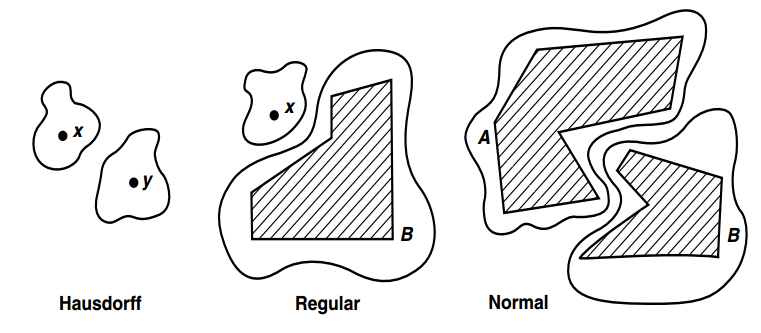
\includegraphics[scale = 0.5]{separation_axioms.png}}
\end{minipage}
\caption{\footnotesize{\textbf{The separation axioms \citep{munkres2000topology}}}}
\label{fig: separation_axioms}
\end{figure}

\item \begin{proposition}
\begin{align*}
T_4 \Rightarrow T_3 \Rightarrow T_2 \Rightarrow T_1
\end{align*}
\end{proposition}

\item \begin{remark} (\emph{\textbf{Separation axioms $\neq$ Discounnected Space}})\\
These axioms are called \emph{\textbf{separation axioms}} for the reason that they involve ``\emph{separating”} certain kinds of \emph{sets from one another} by \emph{\textbf{disjoint open sets}}. 

We have used the word ``\emph{separation}" before, of course, when we studied \emph{connected spaces}. But in that case, we were trying to find \emph{disjoint open sets} \emph{\textbf{whose union was the entire space}}.
\end{remark}

\item \begin{lemma}
Let $X$ be a topological space. Let one-point sets in $X$ be closed.
\begin{enumerate}
\item $X$ is \textbf{regular} if and only if given a point $x$ of $X$ and a neighborhood $U$ of $x$,
there is a \textbf{neighborhood} $V$ of $x$ such that $\bar{V} \subseteq U$.
\item $X$ is \textbf{normal} if and only if given a \textbf{closed} set $A$ and an open set $U$ containing $A$,
there is an \textbf{open set} $V$ containing $A$ such that $\bar{V}\subseteq U$.
\end{enumerate}
\end{lemma}

\item \begin{remark}
$X$ is \emph{\textbf{regular}} $\Leftrightarrow$  Each point of $X$ has a \textbf{\emph{closed neighborhood}}

Note that $X$  is \emph{\textbf{locally compact Hausdorff}} $\Leftrightarrow$ Each point of $X$ has a \textbf{\emph{precompact neighborhood}} i.e. it has a closed neighborhood and \emph{the closure is compact}.
\end{remark}

\item \begin{proposition} (\textbf{Simply Ordered Set is Hausdorff}) \citep{munkres2000topology} \\
Every \textbf{simply ordered set} is a \textbf{Hausdorff} space in the \textbf{order topology}. 
\end{proposition}

\item \begin{proposition} (\textbf{Order Topology is Regular}) \citep{munkres2000topology} \\
Every \textbf{order topology} is a \textbf{regular}. 
\end{proposition}

\item \begin{remark}
It can be shown actually that every \textbf{\emph{order topology}} is a \textbf{\emph{normal}}, which includes all of these two previous results.
\end{remark}

\item 
\begin{proposition} 
(\textbf{Preservation of Hausdorff and Regular Axioms})
\begin{enumerate}
\item The \textbf{product} of two Hausdorff/regular spaces is a Hausdorff/regular space. 
\item A \textbf{subspace} of a Hausdorff/regular space is a Hausdorff/regular space.
\end{enumerate}
\end{proposition}

\item \begin{example} (\emph{\textbf{$\bR_{K}$ is Hausdorff but Not Regular}})\\
The space $\bR_K$ is \emph{\textbf{Hausdorff}} but \emph{\textbf{not regular}}. Recall that $\bR_K$ denotes the reals
in the topology having as \emph{basis all open intervals $(a, b)$ and all sets of the form $(a, b) \setminus K$},
where $K = \set{1/n: n \in \bZ_{+}}$. This space is \emph{Hausdorff}, because any two distinct points have
\emph{disjoint open intervals} containing them.

But it is \emph{\textbf{not regular}}. The set $K$ is \emph{\textbf{closed}} in $\bR_K$ , and it does \emph{not contain the point $0$}.
Suppose that there exist \emph{disjoint open sets} $U$ and $V$ containing $0$ and $K$, respectively.
Choose a basis element containing $0$ and lying in $U$. It must be a basis element of the form $(a, b) \setminus K$, since each basis element of the form $(a, b)$ containing $0$ intersects $K$. Choose $n$ large enough that $1/n \in (a, b)$. Then choose a basis element about $1/n$ contained in $V$;
it must be a basis element of the form $(c, d)$. Finally, choose $z$ so that $z < 1/n$ and $z > \max\set{c, 1/(n + 1)}$. Then $z$ belongs to both $U$ and $V$, so they are not disjoint. \qed
\end{example}

\item \begin{example}(\emph{\textbf{$\bR_{\ell}$ is Normal}})\\
The space $\bR_{\ell}$ is \emph{\textbf{normal}}. Recall that $\bR_{\ell}$ is $\bR$ with \emph{\textbf{lower limit topology}}. (i.e. the basis element is \emph{the half-interval} $[a, b)$.) It is immediate that \emph{one-point sets are closed} in $\bR_{\ell}$, since the topology of $\bR_{\ell}$ is \emph{finer} than that of $\bR$. 

To check \emph{\textbf{normality}}, suppose that $A$ and $B$ are \emph{disjoint closed sets} in $\bR_{\ell}$. For each point $a$ of $A$ choose a basis element $[a, x_a)$ \emph{not intersecting} $B$; and for each point $b$ of $B$ choose a basis element $[b, x_b)$ \emph{not intersecting} $A$.
The open sets
\begin{align*}
U = \bigcup_{a\in A}[a, x_a)\quad \text{ and }\quad V = \bigcup_{b \in B}[b, x_b)
\end{align*}
are \emph{\textbf{disjoint open sets}} about $A$ and $B$, respectively. \qed
\end{example}

\item \begin{example} (\emph{\textbf{The Sorgenfrey plane $\bR_{\ell}^2$ is Not Normal}})\\
The space $\bR_{\ell}$ is regular, so the product space $\bR_{\ell}^2$ is regular. Thus this example serves \emph{two purposes}. It shows that \emph{\textbf{a regular space need not be normal}}, and it shows that \emph{\textbf{the product of two normal spaces need not be normal}}.
\end{example}

\item \begin{definition} (\emph{\textbf{Perfect Map}})\\
A \emph{\textbf{closed} \textbf{continuous} \textbf{surjective} map} $p : X \rightarrow Y$ is called a \underline{\emph{\textbf{perfect map}}} if $p^{-1}(\set{y})$ is
\emph{\textbf{compact}} for each $y \in Y$.
\end{definition}

\item \begin{remark}
\emph{A perfect map} is a \emph{quotient map}.
\end{remark}

\item \begin{proposition}  (\textbf{Preservation Properties of Perfect Map}) \citep{munkres2000topology}\\
Let $p : X \rightarrow Y$ be a \textbf{perfect map}, i.e. it is a \textbf{closed continuous surjective} map who preimage of one point set is \textbf{compact}. Then
\begin{enumerate}
\item If $X$ is \textbf{Hausdorff}, then so is $Y$.
\item If $X$ is \textbf{regular}, then so is $Y$.
\item If $X$ is \textbf{locally compact}, then so is $Y$.
\item If $X$ is \textbf{second-countable}, then so is $Y$.
\end{enumerate}
\end{proposition}

\item \begin{theorem} (\textbf{Preservation Properties of Orbit Space}) \citep{munkres2000topology}\\
Let $G$ be a \textbf{compact topological group}; let $X$ be a topological space; let $\alpha$ be an \textbf{action} of $G$ on $X$. The orbit space $X/G$ is the quotient space under equivalence relationship $x \sim \alpha(x)$. 
\begin{enumerate}
\item If $X$ is \textbf{Hausdorff}, then so is $X/G$.
\item If $X$ is \textbf{regular}, then so is $X/G$.
\item If $X$ is \textbf{normal}, then so is $X/G$.
\item If $X$ is \textbf{locally compact}, then so is $X/G$.
\item If $X$ is \textbf{second-countable}, then so is $X/G$.
\end{enumerate}
\end{theorem}

\end{itemize}
\subsection{Normal Spaces}
\begin{itemize}
\item \begin{remark}
As we have seen, unlike its name suggested, normal spaces are \emph{not as well-behaved} as one might wish.  On the other hand, \emph{\textbf{most of the spaces}} with which we are familiar do \emph{satisfy this axiom}, as we shall see. 

Its \emph{\textbf{importance}} comes from the fact that the results one can prove \emph{\textbf{under the hypothesis of \underline{normality}}} are central to much of topology. The \emph{\textbf{Urysohn metrization theorem}} and \emph{\textbf{the Tietze extension theorem}} are two such results
\end{remark}

\item \begin{proposition}  \citep{munkres2000topology} \\
Every \underline{\textbf{locally compact Hausdorff}} space is \textbf{regular}.
\end{proposition}



\item \begin{theorem} (\textbf{Regular $+$ Second-Countable $\Rightarrow$ Normal})\citep{munkres2000topology}\\
Every \underline{\textbf{regular} space with a \textbf{countable basis}} is \textbf{normal}.
\end{theorem}

\item \begin{proposition}   (\textbf{Regular $+$ Lindel{\"o}f $\Rightarrow$ Normal})\citep{munkres2000topology}\\
Every \underline{\textbf{regular Lindel{\"o}f} space} is \textbf{normal}.
\end{proposition}



\item \begin{theorem} \citep{munkres2000topology}\\
Every \underline{\textbf{metrizable}} space is \textbf{normal}.
\end{theorem}


\item \begin{theorem} \citep{munkres2000topology, reed1980methods}\\
Every \underline{\textbf{compact Hausdorff}} space $X$ is \textbf{normal}.
\end{theorem}

\item \begin{theorem} \citep{munkres2000topology}\\
Every \underline{\textbf{well-ordered}} set $X$ is \textbf{normal} in the \textbf{order topology}.
\end{theorem}

In fact, a stronger theorem holds:
\begin{theorem}
Every \textbf{order} topology is normal
\end{theorem}

\item \begin{example} (\emph{\textbf{The Uncountable Product of Normal Spaces Need Not be Normal}})\\ 
If $J$ is \emph{\textbf{uncountable}}, the product space $\bR^{J}$ is \emph{\textbf{not normal}}.  

This example serves \emph{three purposes}. It shows that \underline{\emph{\textbf{a regular space $\bR^{J}$ need not be normal}}}. It shows that \underline{\emph{\textbf{a subspace of a normal space need not be normal}}}, for $\bR^{J}$ is \emph{homeomorphic} to the subspace $(0, 1)^J$ of $[0, 1]^J$, which (assuming \emph{the Tychonoff theorem}) is \emph{\textbf{compact Hausdorff}} and therefore \emph{normal}. And it shows that \emph{\textbf{an \underline{uncountable product} of normal spaces need not be normal}}. It leaves unsettled the question as to whether \emph{a finite or a countable product of normal spaces might be normal}.
\end{example}

\item \begin{example} (\emph{\textbf{The Finite Product of Normal Spaces Need Not be Normal}}).\\
Recall $S_{\Omega} = \{x: x\in X \text{ and } x < \Omega\}$ is the \emph{\textbf{uncountable section}} of a \emph{\textbf{well-ordered set}} $X$ by $\Omega$ where $\Omega$ is the \emph{\textbf{largest element}} of $X$ (called \underline{\emph{\textbf{the minimal uncountable well-ordered set}}}).

Consider \emph{\textbf{the well-ordered set}} $\bar{S}_{\Omega}$, \emph{in the order topology}, and consider the subset $S_{\Omega}$, \emph{in the subspace topology} (which is the same as the order topology). \emph{Both spaces are \textbf{normal}}, but the product space $S_{\Omega}\times \bar{S}_{\Omega}$ is \emph{\textbf{not normal}}.

his example serves \emph{three purposes}. First, it shows that \underline{\emph{\textbf{a regular space need not be normal}}}, for $S_{\Omega}\times \bar{S}_{\Omega}$ is a \emph{product of regular spaces} and therefore regular. Second, it shows that \emph{\textbf{a \underline{subspace of a normal space need not be normal}}}, for $S_{\Omega}\times \bar{S}_{\Omega}$ is a \emph{subspace} of $\bar{S}_{\Omega}\times \bar{S}_{\Omega}$, which is a \emph{\textbf{compact Hausdorff} space} and therefore \emph{\textbf{normal}}. Third, it shows that \emph{\textbf{the \underline{product of two normal spaces need not be normal}}}.
\end{example}
\end{itemize}

\section{Important Theorems}

\subsection{The Urysohn Lemma}
\begin{table}[tb]
\setlength{\abovedisplayskip}{0pt}
\setlength{\belowdisplayskip}{-10pt}
\setlength{\abovedisplayshortskip}{0pt}
\setlength{\belowdisplayshortskip}{0pt}
\footnotesize
\centering
\caption{Comparison the Urysohn Lemma and Geometric Hahn-Banach Theorem}
\label{tab: separation}
%\setlength{\extrarowheight}{1pt}
\renewcommand\tabularxcolumn[1]{m{#1}}
\small
\begin{tabularx}{1\textwidth} { 
  | >{\raggedright\arraybackslash} m{2.5cm}
  | >{\centering\arraybackslash}X
  | >{\centering\arraybackslash}X  | }
 \hline
  &  \emph{Urysohn's Lemma}  & \emph{Geometric Hahn-Banach Theorem}   \\
  \hline \vspace{5pt}
\emph{space}    \vspace{2pt} & \emph{\textbf{normal} topological space $T_4$ }  & \emph{\textbf{normed linear} space} \\
\hline \vspace{5pt}
\emph{weaker space}    \vspace{2pt} & \emph{\textbf{completely regular} topological space}  & \emph{\textbf{locally convex} space} \\
 \hline \vspace{5pt}
\emph{objects}  \vspace{2pt} &  \emph{two \textbf{closed} subsets} $A, B$  & \emph{two \textbf{convex} subsets} $A, B$ \\
 \hline \vspace{5pt}
\emph{separation pre-condition}  \vspace{2pt} &  \emph{\textbf{closed} subsets are \textbf{disjoint} }  & \emph{\textbf{convex} sets are \textbf{disjoint} }   \\
 \hline \vspace{5pt}
\emph{separating function} \vspace{2pt}  &  \emph{\textbf{continuous function $f: X \rightarrow [0,1]$}}  & \emph{\textbf{a hyperplane defined by linear functional $\ell(x) = a$}}  \\
\hline \vspace{5pt}
\emph{conclusion}  \vspace{2pt}  & \emph{two \textbf{closed sets} can be \textbf{separated} by $f$} & \emph{two \textbf{convex sets} can be \textbf{separated} by \textbf{hyperplane}}
    \\
\hline \vspace{5pt}
\emph{conclusion in math} \vspace{2pt}  &  \begin{align*}
f(A) = \set{0}\text{ and }f(B) = \set{1}
\end{align*}  & \begin{align*}
\sup_{a \in A}\ell(a) \le a \le \inf_{b \in B}\ell(b)
\end{align*}   \\
\hline
\end{tabularx}
\end{table}

\begin{itemize}
\item \begin{theorem} (\textbf{Urysohn Lemma}). \citep{munkres2000topology}\\
Let $X$ be a \textbf{normal} space; let $A$ and $B$ be \textbf{disjoint closed subsets} of $X$. Let $[a, b]$ be a \textbf{closed interval} in the real line. Then there exists a \textbf{continuous} map
\begin{align*}
f : X \rightarrow [a, b]
\end{align*}
such that $f(x) = a$ for \textbf{every} $x$ in $A$, and $f(x) = b$ for \textbf{every} $x$ in $B$.
\end{theorem}

\item \begin{corollary} (\textbf{Urysohn Lemma for $G_{\delta}$}). \citep{munkres2000topology}\\
Let $X$ be a \textbf{normal} space. Then there exists a \textbf{continuous} map
\begin{align*}
f : X \rightarrow [0, 1]
\end{align*}
such that $f(x) = 0$ for \textbf{every} $x \in A$, and $f(x) > 0$ for \textbf{every} $x \not\in A$ \textbf{if and only if} $A$ is a $G_{\delta}$ set, i.e. it equal to a countable intersection of open sets in $X$.
\end{corollary}

\item \begin{theorem} (\textbf{Strong Form of Urysohn Lemma}). \citep{munkres2000topology}\\
Let $X$ be a \textbf{normal} space. Then there exists a \textbf{continuous} map
\begin{align*}
f : X \rightarrow [0, 1]
\end{align*}
such that $f(x) = 0$ for $x \in A$, \textbf{and} $f(x) = 1$ for $x \in B$, and $0 < f(x) < 1$ \textbf{otherwise}  \textbf{if and only if} $A$ and $B$ are disjoint closed $G_{\delta}$ set  in $X$.
\end{theorem}

\item \begin{definition} (\emph{\textbf{Separation by Continuous Function}})\\
If $A$ and $B$ are two subsets of the topological space $X$, and if there is a \textbf{continuous} function $f : X \rightarrow [0, 1]$ such that $f(A) = \set{0}$ and $f(B) = \set{1}$, we say that $A$ and $B$ can be \emph{\textbf{\underline{separated} \underline{by a continuous function}}}.
\end{definition}

\item \begin{remark}
\emph{The Urysohn lemma} says that if \emph{every pair of \textbf{disjoint closed sets}} in $X$ can be \emph{separated by disjoint open sets}, then each such pair can be \emph{\textbf{separated by a continuous function}}. The \emph{\textbf{converse}} is trivial, for if $f : X \rightarrow [0, 1]$ is the function, then $f^{-1}([0, 1/2))$ and $f^{-1}((1/2, 1])$ are \emph{disjoint open sets} containing $A$ and $B$, respectively.
\end{remark}

\item \begin{remark} (\emph{\textbf{Separation by Continuous Function} vs \textbf{Separation by Linear Function}})\\
We can compare \emph{the Urysohn lemma} with \emph{the geometric Hahn-Banach theorem} which seperate two \emph{\textbf{convex sets}} with \emph{linear functional}. See Table \ref{tab: separation}. The \emph{geometric Hahn-Banach theorem} can be seen as a generalization of \emph{the Urysohn lemma} in \emph{\textbf{normed linear space}}.
\end{remark}

\item \begin{remark} (\emph{\textbf{Continuous Function in Compact Hausdorff Space}}) \citep{reed1980methods} \\
\emph{The Urysohn lemma} suggests that there are \emph{\textbf{a lot of continuous functions}} in \emph{normal space}.  \emph{The space of all real-valued continuous functions} $\cC_{\bR}(X)$ on a \emph{\textbf{compact Hausdorff space}} $X$ (which is normal space) has a \emph{\textbf{dense subset}} since any real-valued continuous functions on $[0,1]$ is a \emph{uniform limit} of \emph{\textbf{polynomials}}.  
\end{remark}


\item \begin{definition} (\emph{\textbf{Completely Regular}})\\
A space $X$ is \emph{\textbf{\underline{completely regular}}} if \emph{one-point sets} are \emph{closed} in $X$ and if for each point $x_0$ and each \emph{\textbf{closed}} set $A$ not containing $x_0$, there is a \emph{\textbf{continuous function}} $f : X \rightarrow [0, 1]$ such that $f(x_0) = 1$ and $f(A) = \set{0}$.
\end{definition}

\item \begin{remark}
\begin{align*}
\text{normal } \Rightarrow \text{ completely regular } \Rightarrow \text{regular}
\end{align*}

\item \begin{proposition}
A \textbf{subspace} of a completely regular space is completely regular. 

A \textbf{product} of completely regular spaces is completely regular.
\end{proposition}
\end{remark}

\item \begin{example} (\emph{\textbf{$S_{\Omega}\times \bar{S}_{\Omega}$ is Completely Regular but Not Normal}}).\\
$S_{\Omega}\times \bar{S}_{\Omega}$ is \emph{\textbf{not normal}} but it is the product space of two completely regular spaces.
\end{example}

\item \begin{theorem}  (\textbf{Urysohn Lemma, Locally Compact Version}). \citep{folland2013real}\\ 
Let $X$ be a \textbf{locally compact Hausdorff} space and $K \subseteq U \subseteq X$ where $K$ is \textbf{compact} and $U$ is \textbf{open}.  Then there exists a \textbf{continuous} map
\begin{align*}
f : X \rightarrow [0, 1]
\end{align*}
such that $f(x) = 1$ for \textbf{every} $x \in K$, and $f(x) = 0$ for $x$ outside a \textbf{compact subset} of $U$.
\end{theorem}

\item \begin{corollary}\citep{folland2013real}\\ 
Every \textbf{locally compact Hausdorff} space is \textbf{completely regular}.
\end{corollary}


\item \begin{remark} (\emph{\textbf{Dual Space of $\cC_{c}(X)$ on Locally Compact Hausdorff Space}}) \citep{reed1980methods, folland2013real} \\
The famous \emph{\textbf{Riesz-Markov theorem}} shows that  the \emph{\textbf{dual space}} of $\cC_{c}(X)$, the space of compactly supported continuous function on \emph{locally compact Hausdorff space} $X$ is isomorphic to \underline{\emph{the space of \textbf{signed regular Borel measures}}} on $X$, i.e. $(\cC_c(X))^{*} \simeq \cM(X)$. The proof of \emph{the Riesz-Markov theorem} is based on \emph{\textbf{the Urysohn lemma} for locally compact space}.
\end{remark}
\end{itemize}

\subsection{The Urysohn Metrization Theorem}
\begin{itemize}
\item \begin{theorem} (\textbf{Urysohn Metrization Theorem}). \citep{munkres2000topology}\\
Every \textbf{regular} space $X$ with a \textbf{countable basis} is \textbf{metrizable}.
\end{theorem}

\item \begin{theorem} (\textbf{Embedding Theorem}).  \citep{munkres2000topology}\\
Let $X$ be a space in which one-point sets are closed. Suppose that $\{f_{\alpha}\}_{\alpha \in J}$ is an indexed family of \textbf{continuous} functions $f_{\alpha}: X \rightarrow \bR$ satisfying the requirement that for each point $x_0$ of $X$ and each neighborhood $U$ of $x_0$, there is an index $\alpha$ such that $f_{\alpha}$ is \textbf{positive} at $x_0$ and \textbf{vanishes outside $U$}. Then the function $F : X \rightarrow \bR^J$ defined by
\begin{align*}
F(x) = \paren{f_{\alpha}(x)}_{\alpha \in J}
\end{align*}
is a \underline{\textbf{topological embedding}} of $X$ in $\bR^J$ . If $f_{\alpha}$ maps $X$ into $[0, 1]$ for each α$\alpha$  then $F$ \textbf{embeds} $X$ in
$[0, 1]^J$.
\end{theorem}

\item \begin{definition} (\emph{\textbf{Separation} of \textbf{Points} From \textbf{Closed} Set by \textbf{Continuous} Functions})\\
\emph{\textbf{A family of continuous functions}} that satisfies the hypotheses of \emph{the embedding theorem above} is said to \emph{\textbf{separate points from closed sets in $X$}}. 

The existence of such a family is readily seen to be \emph{equivalent}, for a space $X$ in which one-point sets are \emph{closed}, to the requirement that $X$ be \emph{completely regular}.
\end{definition}

\item \begin{corollary} (\textbf{Embedding Equivalent Definition} of \textbf{Completely Regular}) \citep{munkres2000topology}\\
A space $X$ is \textbf{completely regular} \textbf{if and only if} it is \textbf{homeomorphic} to a subspace of $[0, 1]^J$ for some $J$.
\end{corollary}
\end{itemize}


\subsection{The Tietze Extension Theorem}
\begin{itemize}
\item \begin{theorem} (\textbf{Tietze Extension Theorem}) \citep{munkres2000topology, reed1980methods}\\
Let $X$ be a \textbf{normal space}; let $A$ be a \textbf{closed subspace} of $X$.
\begin{enumerate}
\item Any \textbf{continuous} map of $A$ into the \textbf{closed interval} $[a, b]$ of $\bR$ may be \textbf{extended}
to a \textbf{continuous} map of \textbf{all of $X$} into $[a, b]$.
\item Any \textbf{continuous} map of $A$ into $\bR$ may be \textbf{extended} to a \textbf{continuous} map of \textbf{all of $X$} into $\bR$.
\end{enumerate}
\end{theorem}

%\item \begin{theorem} (\textbf{Tietze Extension Theorem}) \citep{munkres2000topology, reed1980methods}\\
%Let $X$ be a \textbf{compact} space and let $Y \subset X$ be \textbf{closed}. Let $f$ be any \textbf{continuous real-valued function} on $Y$.
%Then there is a \textbf{continuous} real-valued function $\widetilde{f} \in \cC_{\bR}(X)$ so that $f(y) = \widetilde{f}(y)$ for all $y \in Y$.
%\end{theorem}
\item \begin{theorem} (\textbf{Tietze Extension Theorem, Locally Compact Version}) \citep{folland2013real}\\
Let $X$ be a \textbf{locally compact Hausdorff space}; let $K$ be a \textbf{compact subspace} of $X$. If $f \in \cC(K)$ is a \textbf{continuous} map of $K$ into $\bR$,   there exists a \textbf{continuous} extension $F \in \cC(X)$ of \textbf{all of $X$} into $\bR$ such that $F|_{K} = f$. Moreover, $F$ may be taken to \textbf{vanish}\textbf{ outside a compact set}.
\end{theorem} 

\item \begin{remark} (\emph{\textbf{Extension of Continuous Function vs. Extension of Linear Functional}})\\
We can compare \emph{the Tietze extension theorem} with \emph{the Hahn-Banach theorem} in normed linear space. See from Table \ref{tab: extension} that the Hahn-Banach theorem generalize the Tietze extension theorem from normal topological space to the normed linear space (which is metrizable so normal).
\end{remark}
\end{itemize}
\begin{table}[t]
\setlength{\abovedisplayskip}{0pt}
\setlength{\belowdisplayskip}{-10pt}
\setlength{\abovedisplayshortskip}{0pt}
\setlength{\belowdisplayshortskip}{0pt}
\footnotesize
\centering
\caption{Comparison Tietze Extension Theorem and Hahn-Banach Theorem}
\label{tab: extension}
%\setlength{\extrarowheight}{1pt}
\renewcommand\tabularxcolumn[1]{m{#1}}
\small
\begin{tabularx}{1\textwidth} { 
  | >{\raggedright\arraybackslash} m{3cm}
  | >{\centering\arraybackslash}X
  | >{\centering\arraybackslash}X  | }
 \hline
  &  \emph{\textbf{Tietze Extension Theorem}} & \emph{\textbf{Hahn-Banach Theorem}}   \\
  \hline \vspace{5pt}
\emph{space}    \vspace{2pt} & \emph{\textbf{normal} topological space $T_4$ }  & \emph{\textbf{normed} \textbf{linear} space} \\
 \hline \vspace{5pt}
\emph{subspace}  \vspace{2pt} &  \emph{\textbf{topological} subspace}  & \emph{\textbf{linear} subspace}  \\
 \hline \vspace{5pt}
\emph{function to be extended} \vspace{2pt}  &  \emph{\textbf{real-valued continuous function }}  & \emph{\textbf{linear functional}}  \\
\hline \vspace{5pt}
\emph{additional constraint}  \vspace{2pt}  & \emph{the subspace is \textbf{closed}}    & \emph{the functional \textbf{bounded above by a sublinear functional}}  \\
\hline \vspace{5pt}
\emph{conclusion}  \vspace{2pt}  & \emph{the domain of continuous function can be \textbf{extended to entire space}}    & \emph{the domain of linear functional can be \textbf{extended to entire space}}  \\
\hline
\end{tabularx}
\end{table}

\section{Embeddings of Manifolds}

\newpage
\section{Summary of Preservation of Topological Properties}
\begin{table}[h!]
\setlength{\abovedisplayskip}{0pt}
\setlength{\belowdisplayskip}{-10pt}
\setlength{\abovedisplayshortskip}{0pt}
\setlength{\belowdisplayshortskip}{0pt}
\footnotesize
\centering
\caption{Summary of Preservation of Topological Properties Under Transformations}
\label{tab: preservation}
%\setlength{\extrarowheight}{1pt}
\renewcommand\tabularxcolumn[1]{m{#1}}
\small
\begin{tabularx}{1\textwidth} { 
  | >{\raggedright\arraybackslash} m{3cm}
  | >{\centering\arraybackslash}X
  | >{\centering\arraybackslash}X
  | >{\centering\arraybackslash}X  | }
 \hline
  &  \emph{\textbf{subspace}} &  \emph{\textbf{product space}} &  \emph{\textbf{image of continuous function}}   \\
  \hline \vspace{5pt}
\emph{\textbf{connected}}  \vspace{2pt} & $\checkmark$  &  if finite product, $\checkmark$; if countable product, $\checkmark$ under product topology  &   $\checkmark$  \\
\hline \vspace{5pt}
\emph{\textbf{locally connected}}  \vspace{2pt} & if \emph{\textbf{open and connected}} subspace, $\checkmark$  & if \emph{\textbf{all but finitely many} of spaces are \textbf{connected}},  $\checkmark$  & in general  $\times$  \\
 \hline \vspace{5pt}
\emph{\textbf{compact}}  \vspace{2pt} & if \emph{\textbf{closed}} subspace, $\checkmark$;  & for \emph{\textbf{arbitrary}} product, $\checkmark$ & $\checkmark$ \\
 \hline \vspace{5pt}
\emph{\textbf{locally compact}}  \vspace{2pt} & if \emph{\textbf{closed} or \textbf{open}} subspace and Hausdorff, $\checkmark$  & if \emph{\textbf{finite}} product, $\checkmark$; if infinite product $\times$ & if $f$ is a \emph{\textbf{perfect map}}, then $\checkmark$; in general $\times$ \\
 \hline \vspace{5pt}
\emph{\textbf{first-countable}} \vspace{2pt}  &  $\checkmark$ & if \emph{\textbf{countable}} product, $\checkmark$ &  if $f$ is a \emph{\textbf{open map}}, then $\checkmark$; in general $\times$ \\
\hline \vspace{5pt}
\emph{\textbf{second-countable}}  \vspace{2pt}  &  $\checkmark$ & if \emph{\textbf{countable}} product, $\checkmark$ &  if $f$ is a \emph{\textbf{open map or perfect map}}, then $\checkmark$; in general $\times$ \\
\hline \vspace{5pt}
\emph{\textbf{separable}}  \vspace{2pt}  & if metrizable, then $\checkmark$; in general $\times$ & if \emph{\textbf{countable}} product, $\checkmark$  & $\checkmark$\\
\hline \vspace{5pt}
\emph{\textbf{Lindel\"of}}  \vspace{2pt}  & if metrizable, then $\checkmark$; in general $\times$  & $\times$ & $\checkmark$ \\
\hline \vspace{5pt}
\emph{\textbf{$T_1$ axiom}}  \vspace{2pt}  &  $\checkmark$ & for \emph{\textbf{arbitrary}} product, $\checkmark$ &  in general $\times$ \\
\hline \vspace{5pt}
\emph{\textbf{Hausdorff $T_2$}}  \vspace{2pt}   & $\checkmark$  & for \emph{\textbf{arbitrary}} product, $\checkmark$ & if $f$ is a \emph{\textbf{perfect map}}, then $\checkmark$; in general $\times$ \\
\hline \vspace{5pt}
\emph{\textbf{regular $T_3$}}  \vspace{2pt}  & $\checkmark$  & for \emph{\textbf{arbitrary}} product, $\checkmark$ & if $f$ is a \emph{\textbf{perfect map}}, then $\checkmark$ ; in general $\times$ \\
\hline \vspace{5pt}
\emph{\textbf{completely regular}}  \vspace{2pt}  & $\checkmark$  & for \emph{\textbf{arbitrary}} product, $\checkmark$ & in general $\times$ \\
\hline \vspace{5pt}
\emph{\textbf{normal $T_4$}}  \vspace{2pt}  & $\times$  & $\times$ &  $\times$ \\
\hline \vspace{5pt}
\emph{\textbf{paracompact}}  \vspace{2pt}  & if \emph{\textbf{closed}} subspace, $\checkmark$;  &  $\times$  &  $\times$ \\
\hline \vspace{5pt}
\emph{\textbf{topologically complete}}  \vspace{2pt}  & for \emph{\textbf{closed} or \textbf{open}} subspace, $\checkmark$  &  if \emph{\textbf{countable}} product, $\checkmark$  &  $\times$ \\
\hline
\end{tabularx}
\end{table}


\newpage
\section{Summary of Counterexamples for Topological Properties}
\begin{table}[h!]
\setlength{\abovedisplayskip}{0pt}
\setlength{\belowdisplayskip}{-10pt}
\setlength{\abovedisplayshortskip}{0pt}
\setlength{\belowdisplayshortskip}{0pt}
\footnotesize
\centering
\caption{Summary of Counterexamples for Topological Properties}
\label{tab: counterexample}
%\setlength{\extrarowheight}{1pt}
\renewcommand\tabularxcolumn[1]{m{#1}}
\small
\begin{tabularx}{1\textwidth} { 
  | >{\raggedright\arraybackslash} m{2cm}
  | >{\centering\arraybackslash}X
  | >{\centering\arraybackslash}X
  | >{\centering\arraybackslash}X
  | >{\centering\arraybackslash}X
  | >{\centering\arraybackslash}X
  | >{\centering\arraybackslash}X
  | >{\centering\arraybackslash}X
  | >{\centering\arraybackslash}X
  | >{\centering\arraybackslash}X
  | >{\centering\arraybackslash}m{1.5cm}
  | >{\centering\arraybackslash}m{1.5cm}  | }
 \hline
  &  $\bR^{\omega}$  $\srT_{prod}$ &  $\bR^{\omega}$  $\srT_{box}$ &  $\bR^{\omega}$  $ \srT_{unif}$ &  $\bR_{K}$  &  $\bR_{\ell}$ & $\bR_{\ell}^2$  & $I_o^2$  & $S_{\Omega}$ & $\bar{S}_{\Omega}$ & $S_{\Omega} \times \bar{S}_{\Omega}$ & $(x,$ $\sin(1/x))$\\
  \hline \vspace{5pt}
\emph{\textbf{connected}}  \vspace{2pt} & $\checkmark$ & $\times$ & $\times$  & $\checkmark$ & $\times$ & $\times$ & $\checkmark$ &  $\times$ & $\times$ &  $\times$ &  $\checkmark$  \\
\hline \vspace{5pt}
\emph{\textbf{path connected}}  \vspace{2pt} & $\checkmark$ & $\times$ &  $\times$ & $\times$ & $\times$ & $\times$ & $\times$ & $\times$ &$\times$  & $\times$ &  $\times$ \\
\hline \vspace{5pt}
\emph{\textbf{locally connected}}  \vspace{2pt} &  $\checkmark$ &  $\times$  &  $\checkmark$ & $\times$ & $\times$ &  $\times$ & $\checkmark$ & $\times$ &$\times$  &  $\times$ &  $\times$ \\
\hline \vspace{5pt}
\emph{\textbf{locally path connected}}  \vspace{2pt} &  $\checkmark$ &  $\times$  &  $\checkmark$ &$\times$ & $\times$ & $\times$ & $\times$ & $\times$ & $\times$ &$\times$ &  $\times$ \\
 \hline \vspace{5pt}
\emph{\textbf{compact}}  \vspace{2pt} & $\times$ & $\times$ & $\times$ & $\times$ & $\times$ & $\times$ & $\checkmark$ &$\times$ & $\checkmark$ & $\times$  & $\checkmark$ \\
 \hline \vspace{5pt}
\emph{\textbf{limit point compact}}  \vspace{2pt} & $\times$  & $\times$ & $\times$ & $\times$  & $\times$& $\times$ &$\checkmark$ &$\checkmark$ & $\checkmark$ &  &  $\checkmark$\\
 \hline \vspace{5pt}
\emph{\textbf{sequentially compact}}  \vspace{2pt} & $\times$ & $\times$ & $\times$ & $\times$  & $\times$& $\times$ & $\checkmark$ & $\checkmark$ & $\checkmark$ &  &  $\checkmark$\\
 \hline \vspace{5pt}
\emph{\textbf{locally compact}}  \vspace{2pt} & $\times$ & $\times$ & $\times$ & $\times$ & $\times$ & $\times$ &  $\checkmark$ &$\checkmark$ & $\checkmark$ & $\checkmark$  & $\checkmark$\\
 \hline \vspace{5pt}
 \emph{\textbf{paracompact}}  \vspace{2pt}   & $\checkmark$ & $\checkmark$ & $\checkmark$ & $\times$ & $\checkmark$ &$\times$  & $\checkmark$ &$\times$ & $\checkmark$ & $\times$  & $\checkmark$ \\
\hline \vspace{5pt}
\emph{\textbf{first-countable}} \vspace{2pt}   & $\checkmark$ & $\times$ & $\checkmark$ & $\checkmark$ & $\checkmark$ & $\checkmark$ & $\checkmark$  & $\checkmark$  & $\times$ & $\times$  & \\
\hline \vspace{5pt}
\emph{\textbf{second-countable}}  \vspace{2pt}   & $\checkmark$ & $\times$ & $\times$& $\checkmark$ & $\times$ & $\times$& $\times$ & $\times$  & $\times$ & $\times$ &  \\
\hline \vspace{5pt}
\emph{\textbf{separable}}  \vspace{2pt}   & $\checkmark$ & $\times$ & $\times$ & $\checkmark$ &$\checkmark$ & $\checkmark$ & $\times$  & $\times$ & $\times$ &  $\times$ & \\
\hline \vspace{5pt}
\emph{\textbf{Lindel\"of}}  \vspace{2pt}   & $\checkmark$ & $\times$ & $\times$ & $\checkmark$ & $\checkmark$ & $\times$  &  $\checkmark$ & $\times$ &  $\checkmark$&  $\times$ &  $\checkmark$ \\
\hline \vspace{5pt}
\emph{\textbf{$T_1$ axiom}}  \vspace{2pt}  & $\checkmark$ & $\checkmark$ & $\checkmark$& $\checkmark$ & $\checkmark$ & $\checkmark$ & $\checkmark$ &$\checkmark$  &  $\checkmark$ & $\checkmark$  & $\checkmark$  \\
\hline \vspace{5pt}
\emph{\textbf{Hausdorff $T_2$}}  \vspace{2pt}  & $\checkmark$ &$\checkmark$  & $\checkmark$ & $\checkmark$ & $\checkmark$ & $\checkmark$ & $\checkmark$  & $\checkmark$  &  $\checkmark$ & $\checkmark$   & $\checkmark$ \\
\hline \vspace{5pt}
\emph{\textbf{regular $T_3$}}  \vspace{2pt}   & $\checkmark$ & $\checkmark$ & $\checkmark$& $\times$  &$\checkmark$ & $\checkmark$ & $\checkmark$  & $\checkmark$  & $\checkmark$  &  $\checkmark$  &  \\
\hline \vspace{5pt}
\emph{\textbf{completely regular}}  \vspace{2pt}   & $\checkmark$ & $\checkmark$ & $\checkmark$ & $\times$  & $\checkmark$ &  $\checkmark$ &  $\checkmark$ & $\checkmark$ &  $\checkmark$ & $\checkmark$  &  \\
\hline \vspace{5pt}
\emph{\textbf{normal $T_4$}}  \vspace{2pt}   & $\checkmark$ & $\checkmark$ & $\checkmark$ & $\times$  & $\checkmark$ & $\times$ & $\checkmark$  & $\checkmark$  & $\checkmark$  & $\times$ &  \\
\hline \vspace{5pt}
\emph{\textbf{locally metrizable}}  \vspace{2pt}   & $\checkmark$ & $\times$ & $\checkmark$ & $\times$  & & &  $\times$  &$\checkmark$  & $\times$  &  $\times$ &  \\
\hline \vspace{5pt}
\emph{\textbf{metrizable}}  \vspace{2pt}   & $\checkmark$ & $\times$ & $\checkmark$ & $\times$  & $\times$ & $\times$&  $\checkmark$ & $\times$ & $\times$  &  $\times$  & $\times$ \\
\hline
\end{tabularx}
\end{table}

\begin{enumerate}
\item $(\bR^{\omega}, \srT_{prod})$: space of \emph{\textbf{countable infinite}} real sequence $(a_n)_{n \in \bZ}$ equipped with \emph{\textbf{product topology}}. Note that under product topology, the \emph{\textbf{basis}} is of form $\prod_{n\in \bZ_{+}}U_n$ where there exists some $N$ so that for all $n \ge N$, $U_n = \bR$.

\item $(\bR^{\omega}, \srT_{box})$: space of \emph{\textbf{countable infinite}} real sequence $(a_n)_{n \in \bZ}$ equipped with \emph{\textbf{box topology}}. Note that under box topology, the \emph{\textbf{basis}} is of form $\prod_{n\in \bZ_{+}}U_n$ where $U_n \neq \bR$ for all $n$.

\item $(\bR^{\omega}, \srT_{unif})$: space of \emph{\textbf{countable infinite}} real sequence $(a_n)_{n \in \bZ}$ equipped with \emph{\textbf{uniform topology}}. Note that the uniform topology is induced by \emph{\textbf{the uniform metric}} $\bar{\rho}$ on $\bR^{\omega}$, which is defined by the equation
\begin{align*}
\bar{\rho}((x_n)_{n \in \bZ_{+}}, (y_n)_{n \in \bZ_{+}}) &= \sup\set{\bar{d}(x_{n}, y_{n}): n \in \bZ_{+}},
\end{align*}
where $\bar{d}$ is \emph{\textbf{the standard bounded metric}} on $\bR$.

\item $\bR_{K}$: the real line $\bR$ equipped with the \emph{\textbf{$K$-topology}}. The $K$-topology is \emph{\textbf{generated}} by \emph{all open intervals} $(a, b)$ \textbf{and} \emph{all sets \textbf{of the form}} 
\begin{align*}
(a,b) \setminus K\text{ where }K = \set{1/n: n \in \bZ_{+}}.
\end{align*}

\item $\bR_{\ell}$: the real line $\bR$ equipped with the \emph{\textbf{lower limit topology}}. The basis of lower limit topology is  the collection of all \emph{\textbf{half-open intervals}} of the form
\begin{align*}
[a,b) = \{x: a \le  x < b\},
\end{align*} where $a < b$. $\bR_{\ell}$ is also called \emph{\textbf{the Sorgenfrey line}}.

\item $\bR_{\ell}^2 = \bR_{\ell} \times \bR_{\ell}$: is called \emph{\textbf{the Sorgenfrey plane}}.

\item $I_o^2$: is called \emph{\textbf{ordered square}} where $I = [0,1]$. It is the set $[0,1] \times [0,1]$ in \emph{\textbf{the dictionary order topology}}. In dictionary order relationship, $(x_1, x_2) < (y_1, y_2)$ if and only if $x_1 < y_1$ or $(x_1 = y_1) \land (x_2 < y_2)$. In dictionary order topology, open intervals are of the form 
\begin{align*}
\set{(x_1, x_2): x_1 \in (a, b) \text{ or } (x_1 = c) \land (x_2 \in (d, e))} = ((a, b) \times I) \cup (c \times (d, e)).
\end{align*}

\item $S_{\Omega}$: is \emph{\textbf{the uncountable ordinal space}}. If $A$ is a \emph{\textbf{well-ordered set}} then $A$ itself contains a \emph{\textbf{smallest element}} which we will denote by $a_0$. For each element $x$ in a \emph{well-ordered set} $A$, \emph{\textbf{the section at $x$}} is defined to be the subset
\begin{align*}
S_x = (-\infty, x) = [a_0, x) = \set{y \in A:  y < x}.
\end{align*} \emph{The uncountable ordinal space} $S_{\Omega}$ is \emph{an \textbf{uncountable well-ordered set}} in which \emph{each
section $S_x$ is \textbf{countable}}. This description of $S_{\Omega}$  is justified by the following:
\begin{lemma}
There exists an uncountable well-ordered set $A$ such that $S_x$ is countable for each $x \in A$, and any two uncountable well-ordered sets satisfying this property are \textbf{order isomorphic} (that is, they have the same order type).
\end{lemma}

\item $\bar{S}_{\Omega}$:  is \emph{\textbf{the closed uncountable ordinal space}}. It is defined by $\bar{S}_{\Omega} = S_{\Omega} \cup \set{\Omega}$ with \emph{\textbf{the well-ordering}} given by: (a) if $x, y \in S_{\Omega}$ then $x < y$ in $\bar{S}_{\Omega}$ iff $x < y$ in $S_{\Omega}$, and (b) if $x \in S_{\Omega}$ then $x < \Omega$. Notice that $ \Omega$ is a \emph{\textbf{maximal element}} in $\bar{S}_{\Omega}$ (but $S_{\Omega}$ \emph{does not have a maximal element}). $S_{\Omega}$ is the section of $\Omega$ in $\bar{S}_{\Omega}$.

\item $S_{\Omega} \times \bar{S}_{\Omega}$

\item $\bar{S}$: is called  \emph{\textbf{the topologist's sine curve}}. It is the closure of the graph
\begin{align*}
S = \set{(x, \sin(1/x)): 0 < x \le 1}.
\end{align*} That is $\bar{S} = S \cup \set{(x,y): x=0}$.

\end{enumerate}

\newpage
\bibliographystyle{plainnat}
\bibliography{book_reference.bib}
\end{document}